\chapter{Web Application}\label{chap:web_app}

In this section, we will describe the proposed web application for novel song recommendation. The section is structured as follows: 
\begin{itemize}
    \item In Section \ref{sec:analysis} we analyze our application goals and describe what the user can expect from our application.
    \item In Section \ref{sec:implementation} We briefly introduce the building blocks of our application with focus on the individual similarity measures implementation and calculation of recommendations.
    \item In Section \ref{sec:configurations} We present the possible configurations of our application.
    \item In Section \ref{sec:user_docs} we provide user documentation for our web application.
\end{itemize}

\section{Analysis}\label{sec:analysis}

There are many music recommendation web applications online such as Youtube\footnote{www.youtube.com}, Spotify\footnote{www.spotify.com}etc. They have a lot of data about users, user activity, a lot of songs, a lot of tags. Our application is just a small project that does not aspire on growing to such extend. What we want to provide to our users are not endless playlists but more of an inspiration to find new songs and then play them (for exapmle on Youtube). \\
We obviously want this application to have the usual web application functionalities, such as creating accounts, logging in and out, going through different web pages, etc. Because it is a song recommender application, we want our users to be able to view recommendations, create playlists, search for songs and like and dislike songs to improve the suggestions for him. Besides that we want the users to be able to add songs they already know and that are missing in our database and then see, which songs are similar to it based on various recommendation methods. Even if the does not like the recommended song, it might be interesting for him to see, which songs are similar to it based on for example lyrics. It gives the user a more hands on experience and is so not only about music but also a bit about the theory of this application. \\

\section{Implementation}\label{sec:implementation}
In this section, we present the overall architecture of our application with focus on the recommendation functionalities which are described in more detail in Subsections \ref{ssec:measure_implementation}, \ref{ssec:method_selection} and \ref{ssec:recom_calcs}. 

\subsection{Technologies}

We build our web application in the Django framework in Python 3.6. We chose Python because it is well suited for machine learning and Django because it is a Python based framework. Besides this, to ensure a smooth user experience while performing complex computational tasks, we included Celery\footnote{http://www.celeryproject.org} which is a asynchronous task queue to run expensive tasks in the background. We used RabbitMQ\footnote{https://www.rabbitmq.com} as Celery's message broker.

\subsection{Design}

\subsubsection{Models and Database}
For every table in the database, there is a class-based model in the module \texttt{models.py} specifying its features. There is a class of the same name for \texttt{Song} and \texttt{List} tables. The \texttt{Profile} model which is an extension of the build-in Django \texttt{User} model is included to enable specifying the distance of songs to the user and also checking if the user has confirmed his email.\\
 
The class \texttt{Song\_in\_list} keeps track of lists and songs that belong together, the an instance of the \texttt{Played\_song} model specifies a user and a songs he has played. One cannot un-play a song but it can be disliked and it will not appear anymore in recommendations and it will also not be used to calculate recommendations of other songs. \\
There are three different models for storing similarities. They are called \texttt{Distance} whose instances store basic similarities between two songs, \texttt{Distance\_to\_user} whose instances store similarities of a song to a particular list and \texttt{Distance\_to\_user} whose instances store the similarity of a song to a particular user. 
\begin{figure}[ht]
    \centering
	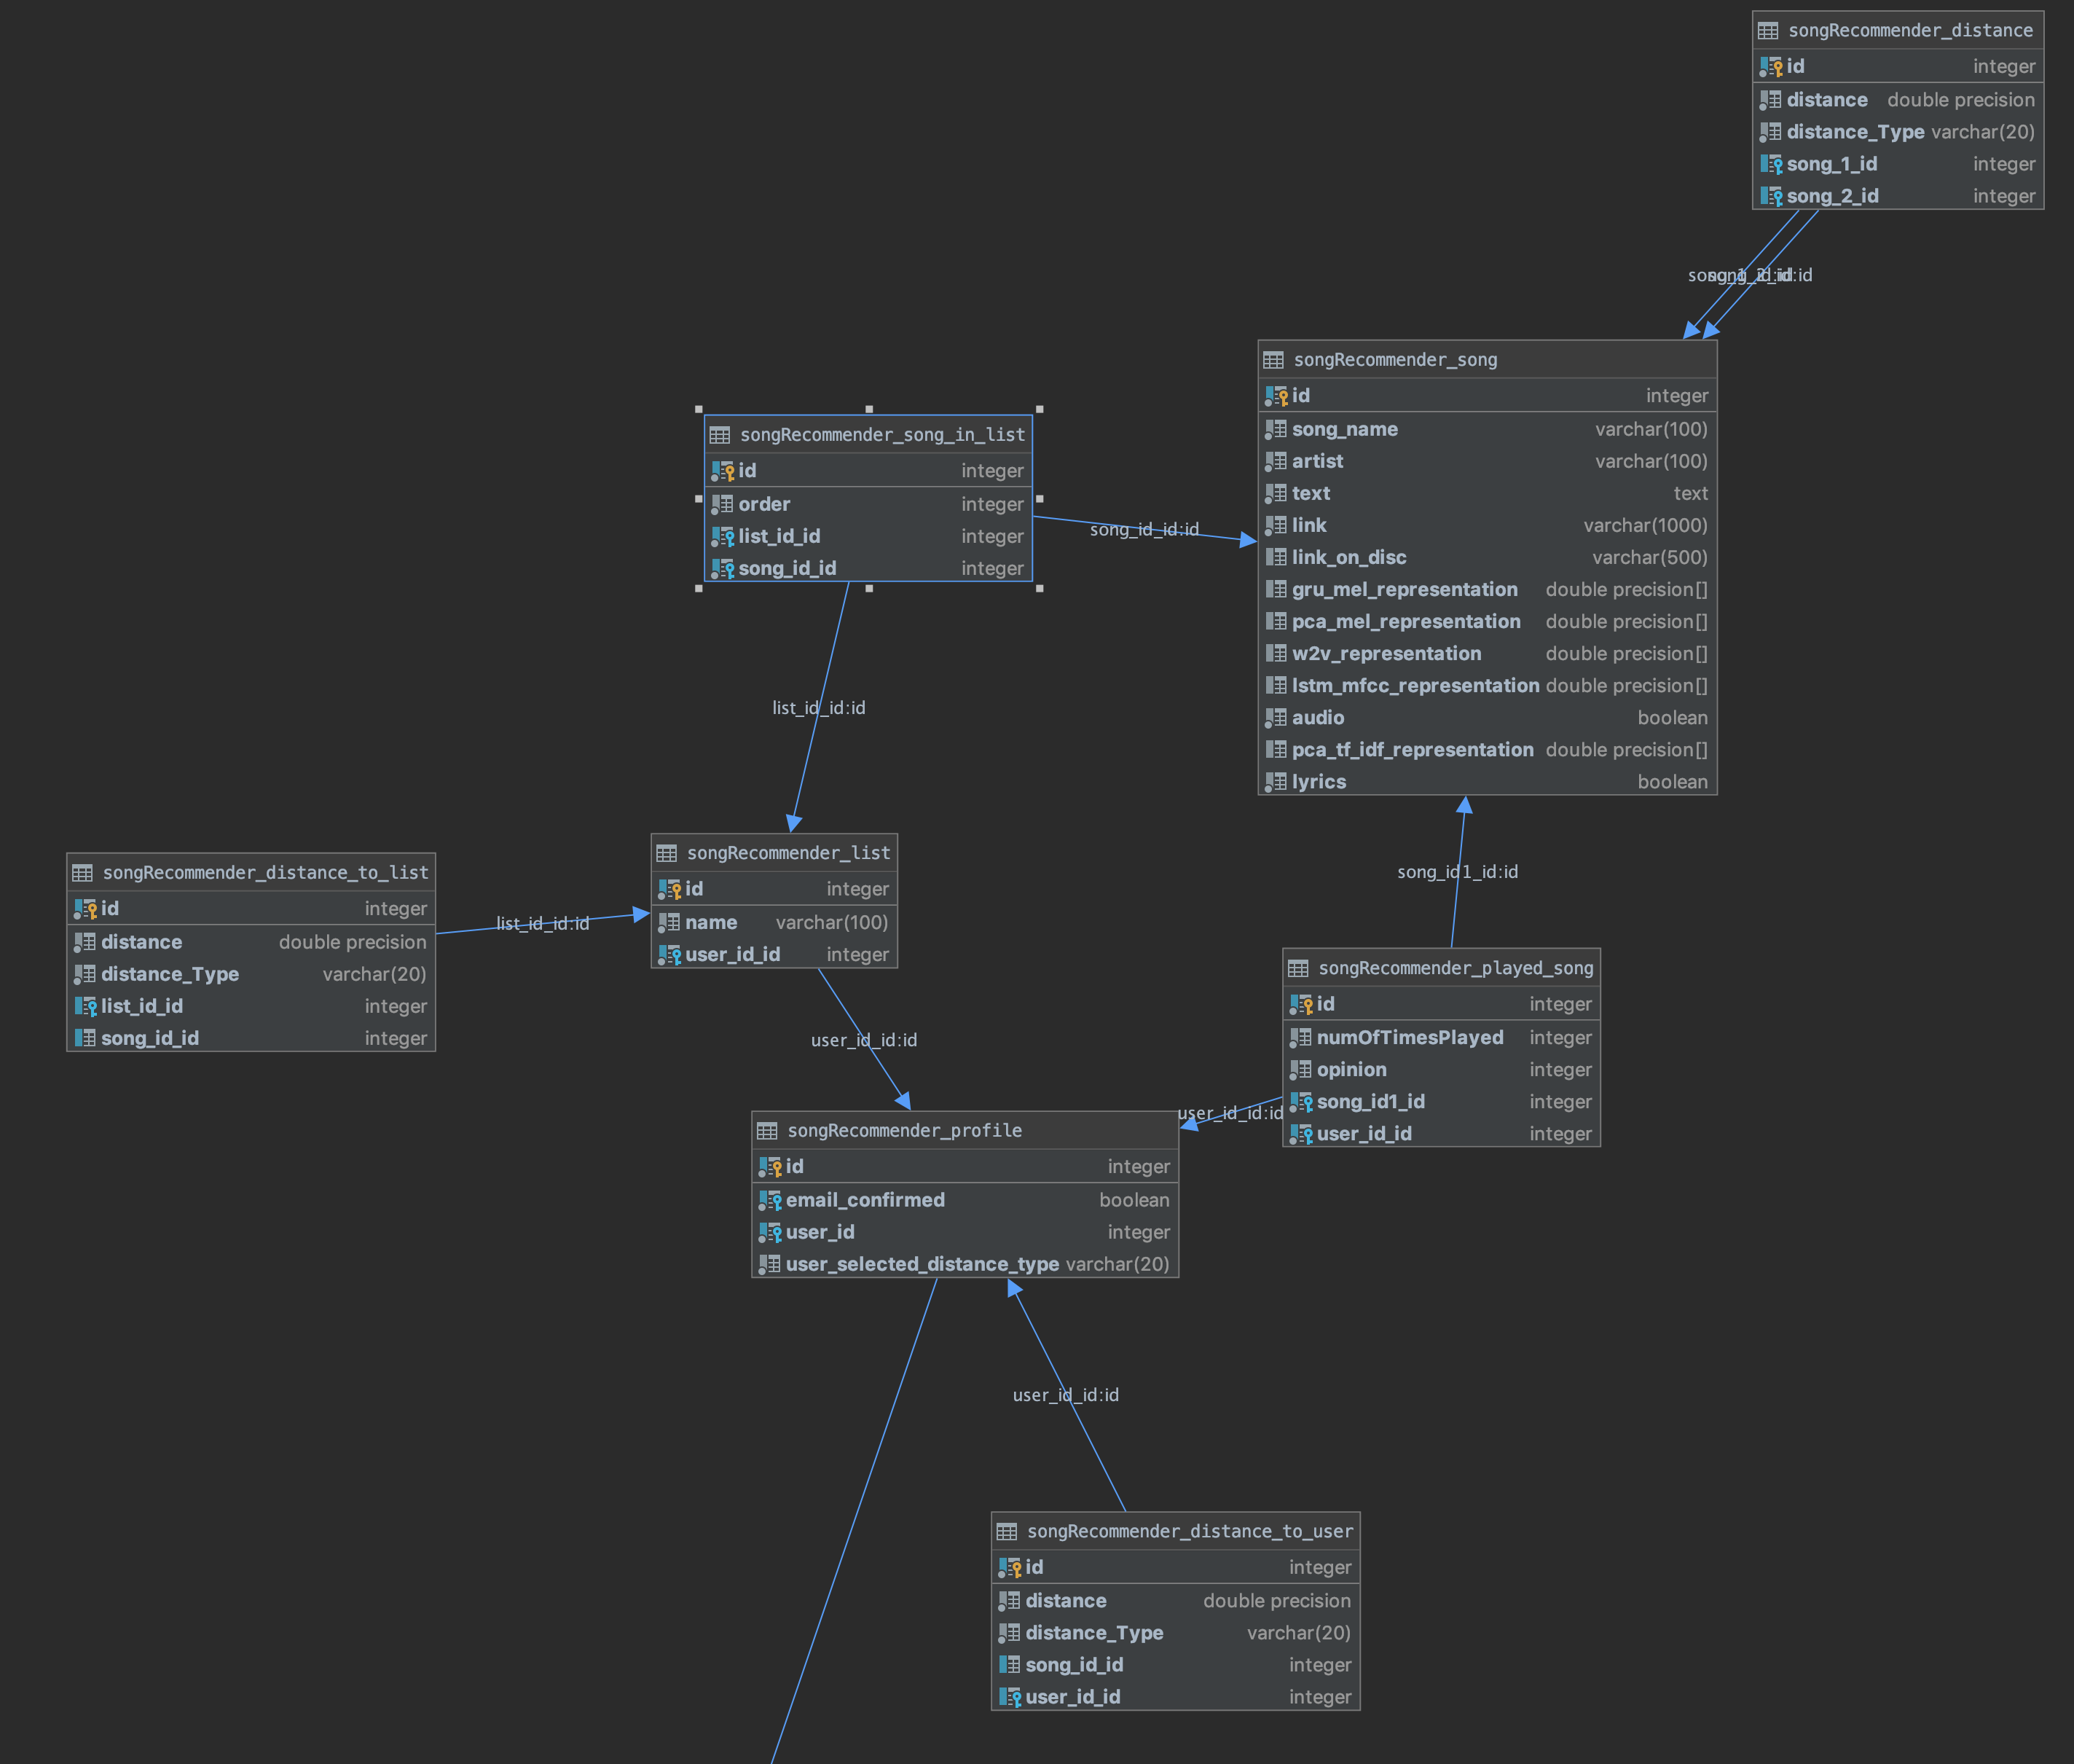
\includegraphics[width=120mm]{./img/postgres_database.png}
	\caption{Diagram of the applications database}
	\label{fig:diagram}
\end{figure}
The database is structured as Figure \ref{fig:diagram} illustrates. Build-in Django tables are omitted for clarity.

\subsubsection{Views}
Views handle the requests users send. Each request from some HTML page is processed by a function from \texttt{views.py}. It takes it request's parameters, calls some functions from the "logic" part of the application if necessary, collects the context for the next HTML page based on that and displays a that page to the user. \\
There are two main kinds of views in this application. First are build-in \textit{class-based views} which are structured around a model class from \texttt{models.py}. For exapmle the \texttt{SongDetailView} is a class-based view. The second are \textit{function-based views} which are not tied to a model. In the application, these are used for example for handling liking and disliking songs. \\
We used both kinds of views as we could make use of the abstraction and code simplification for \textit{class-based views} for most of the pages that revolved around models. The \textit{function based views} on the other hand provided a more flexible choice for functional , not only liking and disliking songs, but also changing the distance metrics etc. \\

\subsubsection{Server}\label{sssec:server}

All the logic of the application is running on the server. Most expensive tasks are sent to Celery to handle them asynchronously so users do not have to wait. \\
The expensive tasks are those that including calculating and recalculating song similarities. They can be triggered by four main events: \\
First is the one when a user adds a new song. The song's mp3 is downloaded from the link the user provides, then the 15 second audio excerpt is created and turned into a mel-spectrogram and MFCC which are then input for audio method models. The songs lyrics are also stripped of punctuation characters and prepared as input for the lyrics methods. This is not the end. The application then calculates the similarity of this song to all the other songs in the database for each measure separately. Afterwards, the similarity of the song to other users and to all the lists in the database is calculated. Adding takes about 15 seconds if there are no othre songs in the database and 555 seconds if the full song dataset is loaded into the database but we only have 1 user with 1 list. \\ 
Secondly, the user can play a song for the second time. We take it as a sign that he likes that song and include it into the distance recalculations for similarities of songs to the user.\\
The third event is adding a song to a list. In that case, the similarities of all songs to this list are recalculated. \\
And the fourth event is liking or disliking a song by a user, which results in recalculating similarities of all songs to this user's taste. \\
These are quite time consuming tasks especially with a growing song, list and user database. \\

\subsubsection{Client}
The client only receives pre-computed HTML5 pages with some CSS for nicer design. There is no computation on his side.

\subsection{Similarity measure implementation}\label{ssec:measure_implementation}

In Chapter \ref{chap:experiments} we did not finalize our method selection, we just summarized their performance results. That is because to implement them, we cannot only look at their performance but also at their computational properties --- time and space complexities. \\

\subsubsection{Time and space complexity}

There are four main events described in \ref{sssec:server} that trigger the songs similarities calculations and recalculations in the application. However only the duration of addition of a new song into the database is dependant on the form of the vector representation. With all the other recalculations we only use the similarities already stored in the database which are represented by a single floating point number. \\

When a new song is added, it is transformed into the respective vectors for each implemented method. And then its similarity to all the songs inside the database has to be calculated which is very dependant on the length of the vector representations. A simple \textit{for cycle} is too time consuming for Python. Therefore, we use the \texttt{sklearn.pairwise.metrics.cosine\_similarity} on the new vector and all the vector representations in the database for each implemented method. It is the same function as we used for calculating similarity matrices for evaluation. However, because the server only has 8GB of RAM and because we expect a growing number of songs inside our database, we might get a memory error if calculating the similarity of the added song to all the songs in the database at once. Because of that, the songs in the database are split into chunks and the similarities are calculated for each chunk, then saved and then the next chunk is processed. \\
The chunk-size differs for different methods. With an increasing chunk-size the similarity calculations are faster so we want to make it as big as possible, however it is smaller for longer vectors and shorter for longer vectors as it is there merely to avoid a memory error. \\
The reason we care about how fast the calculations are is not really to make the next page load faster as the user does not have to wait in any case because of the asynchronous task queue. We however want our application to be responsive and recommend relevant songs as soon as possible, not the next day. \\

The biggest issue with space complexity for methods is the size of their trained model. The models are needed when a new song is added to create the respective song-representation for the particular method. To avoid re-loading the models every time a new song is added, they are loaded into memory once at the beginning when the server starts. For some methods, the models are quite small (tens to hundreds of kilobytes) but for some, their size goes up to Gigabytes. \\
This poses a problem. It takes time to load big models which is the smaller issue as it happens only once in theory. However, some of them are as big as the RAM of the server, which makes predictions much slower and could sometimes even through a memory error exception. It did not happen while testing the application, but that is because it was developed on a computer with 16GB of RAM and then deployed on a different one.

\subsubsection{Method selection}\label{ssec:method_selection}

With keeping the above in mind, let's look at Table \ref{table:time_space_complexities} and Figure \ref{fig:threshold_method_comparison}. We put our final choices together based on these values but there is also a third thing to consider. We put a higher priority on lyric based methods as they are more unique and their recommendations maybe a bit more interesting for the user and we also take the diversity of our methods into account. \\
First we rule out the method that seem to perform badly, are ranked last in most categories. It is SOM\_W2V, GRU\_Spec\_5712, LSTM\_Spec\_5712, and LSTM\_mel, and PCA\_spec\_320. \\
We also will not implement the GRU\_spec\_20400 and LSTM\_spec\_20400 and Tf-idf, raw mel-spectrograms anad MFCCs because of the length of their vectors. The PCA\_spec\_1106 and PCA\_spec\_5712 disqualify because of the size of their models. \\
This leaves us with the W2V, PCA\_Tf-idf, PCA\_mel\_320,GRU\_mel, LSTM\_MFCC and GRU\_MFCC. As we can see, none of these has spectrograms as input so we will not use any spectrogram method. Out of these, the worst one is W2V, however, it is a lyric method and it is very different from all other methods, so we will implement it. We will leave out the GRU\_MFCC as we will still have have the LSTM\_MFCC network methods with the same input and GRU\_MFCC is the second worst after W2V. We could obviously keep all the methods we did not rule out but we want to reduce the number of methods because the distance calculations are not calculated in parallel (although they could be) but one after another so more methods are more complex. \\
Let's recapitulate our method choices:
\begin{itemize}
    \item \textbf{PCA\_Tf-idf} is a lyrics-based method and also the best method we presented so this is a no-brainer.
    \item \textbf{W2V} is also a lyrics-based method, it is the worst from the ones we decided to implement but it has short vectors and a small model and helps with our method diversity.
    \item \textbf{PCA\_mel\_320} is the first audio based method. It appears to be good in the average rank of a song, however, that is not very important for recommendation. Anyway its overall results are average and its time and space complexities very nice.
    \item \textbf{GRU\_mel} is a deep neural network method which performed best between neural networks.
    \item \textbf{LSTM\_MFCC} is another deep neural network method which has two components we have not used in any of our implemented methods, the LSTM layers in its architecture and takes the MFCCs as input. It is unique with good results relative to other methods. 
\end{itemize}

\begin{table}[h]
\centering
\renewcommand{\arraystretch}{1.5}
\begin{tabu} to 1\textwidth {| c || X[c] | X[c] | }
 \hline
 \textbf{method} & \textbf{vector length} & \textbf{model size in KB} \\
 \hline
 raw mel-spectrograms & 130,560 & no model \\
 \hline 
 raw MFCCs & 82,688 & no model \\
 \hline
 Tf-idf & 40,165 & 2,600 \\
 \hline
 PCA on Tf-idf & 4,457 & 1,430,000  \\
 \hline
 W2V & 300 & 251,100 \\
 \hline
 SOM\_W2V & 2 & 358,792 \\
 \hline
 PCA\_spec\_1106 & 1,106 & 7,980,000 \\
 \hline
 PCA\_spec\_320 & 320 & 2,320,000\\
 \hline
 PCA\_mel\_5715 & 5,715 & 5,970,000\\
 \hline
 PCA\_mel\_320 & 320 & 336,300 \\
 \hline
 GRU\_spec\_20400 & 20,400 & 67,000 \\
 \hline
 GRU\_spec\_5712 & 5,712 & 59,000 \\
 \hline
 LSTM\_spec\_20400 & 20,400 & 3700 \\
 \hline
 LSTM\_spec\_5712 & 5,712 & 1003 \\
 \hline
 GRU\_mel & 5,712 & 146 \\
 \hline
 LSTM\_mel & 5,712 & 185 \\
 \hline
 GRU\_MFCC & 5,168 & 48 \\
 \hline
 LSTM\_MFCC & 5,168 & 471 \\
 \hline
 \end{tabu} \\
\caption{The vector length and model size for different methods}
\label{table:time_space_complexities}
\end{table}

\subsubsection{Recommendation calculation}\label{ssec:recom_calcs}

The similarity of two songs is calculated using the cosine similarity with threshold $cos\_sim_t$ as described in Subsection
\ref{ssec:evaluation_measures}. The similarity of a song to a user of list is an addition of similarities. To be specific, the similarity of a song $s_i$ to a user is the $ \sum_{k=0}^{k=n} c*cos\_sim_t(s_i, s_k) $  where $ i \neq k $ and $ s_k $ is a song the user played and $n$ is the number of songs the user has played and $c$ is a constant which is either 1 when the song $s_k$ was played or 2 when $s_k$ was also liked. \\
The displayed recommendations do not include songs the user has already played. It is also possible to see always only the top 10 recommendations, overall, and for a each list. When it comes to a page with a specific song, it does not matter what user is viewing it, it is always the same and displays an audio area where it is possible to play the song and 10 most similar song to this one. There is also a possibility to like it or dislike it.\\ 

\section{Configuration options}\label{sec:configurations}

In this section we will describe the configuration options the application provides. There are some options that influence configuration as well as options to change the server settings. All of the configurations are in the module \texttt{setting.py}

\subsection{Similarity method configurations}
The things that can be set for similarity methods are the thresholds. Right now, the threshold values correspond the to keeping 846294 biggest similarities for each similarity method, meaning, there are about 51*16594 instances of \texttt{Distance} stored in the database for each of the implemented methods. Changing the threshold does not influence the songs that are already in the database. Nevertheless, when a new song is added, potentially more distances will be created if the threshold is lowered or less if its raised. \\
Another thing that can be configured in the \texttt{setting.py} module is the default similarity method that is default for a new user account. The user can then change it once he is logged in but at creation, he is assigned one.

\subsection{Email}
There is a boolean variable called \texttt{EMAIL\_DISABLED} which is set on True by default as there is no email service set up with our application, however if a email service and a domain is provided, it is only necessary to change the \texttt{EMAIL\_DISABLED} variable to False and also delete the \texttt{EMAIL\_BACKEND} and replace it with an email service configuration. If the variable is set to False without configuring an email service, the email is printed inside the console and the user has no way of authenticating his account.

\subsection{Server}

The application has not been completely deployed. It runs on \url{http://acheron.ms.mff.cuni.cz:42009/index/} in debug mode. To actually deploy the application, it is necessary go to \texttt{settings.py} and change the \texttt{Debug} variable to \texttt{False}. Then it is necessary to collect all static files (including all the mp3 files) and tell Django where they are as it stops handling static files itself without the debug mode on.\\
It is also necessary to choose some wsgi, for example \texttt{gunicorn} with \texttt{nginx} or \texttt{apache} as web servers.

\section{User documentation}\label{sec:user_docs}
The application has a navigation menu on top of the page which appears on every page. From there, the user can go to the \textit{Homepage} where he can see the lists he created, and top ten recommendations for him. These recommendations exclude disliked and played songs. The \textit{Homepage} is displayed in Figure \ref{fig:home_page}. \\

\begin{figure}[H]
    \centering
	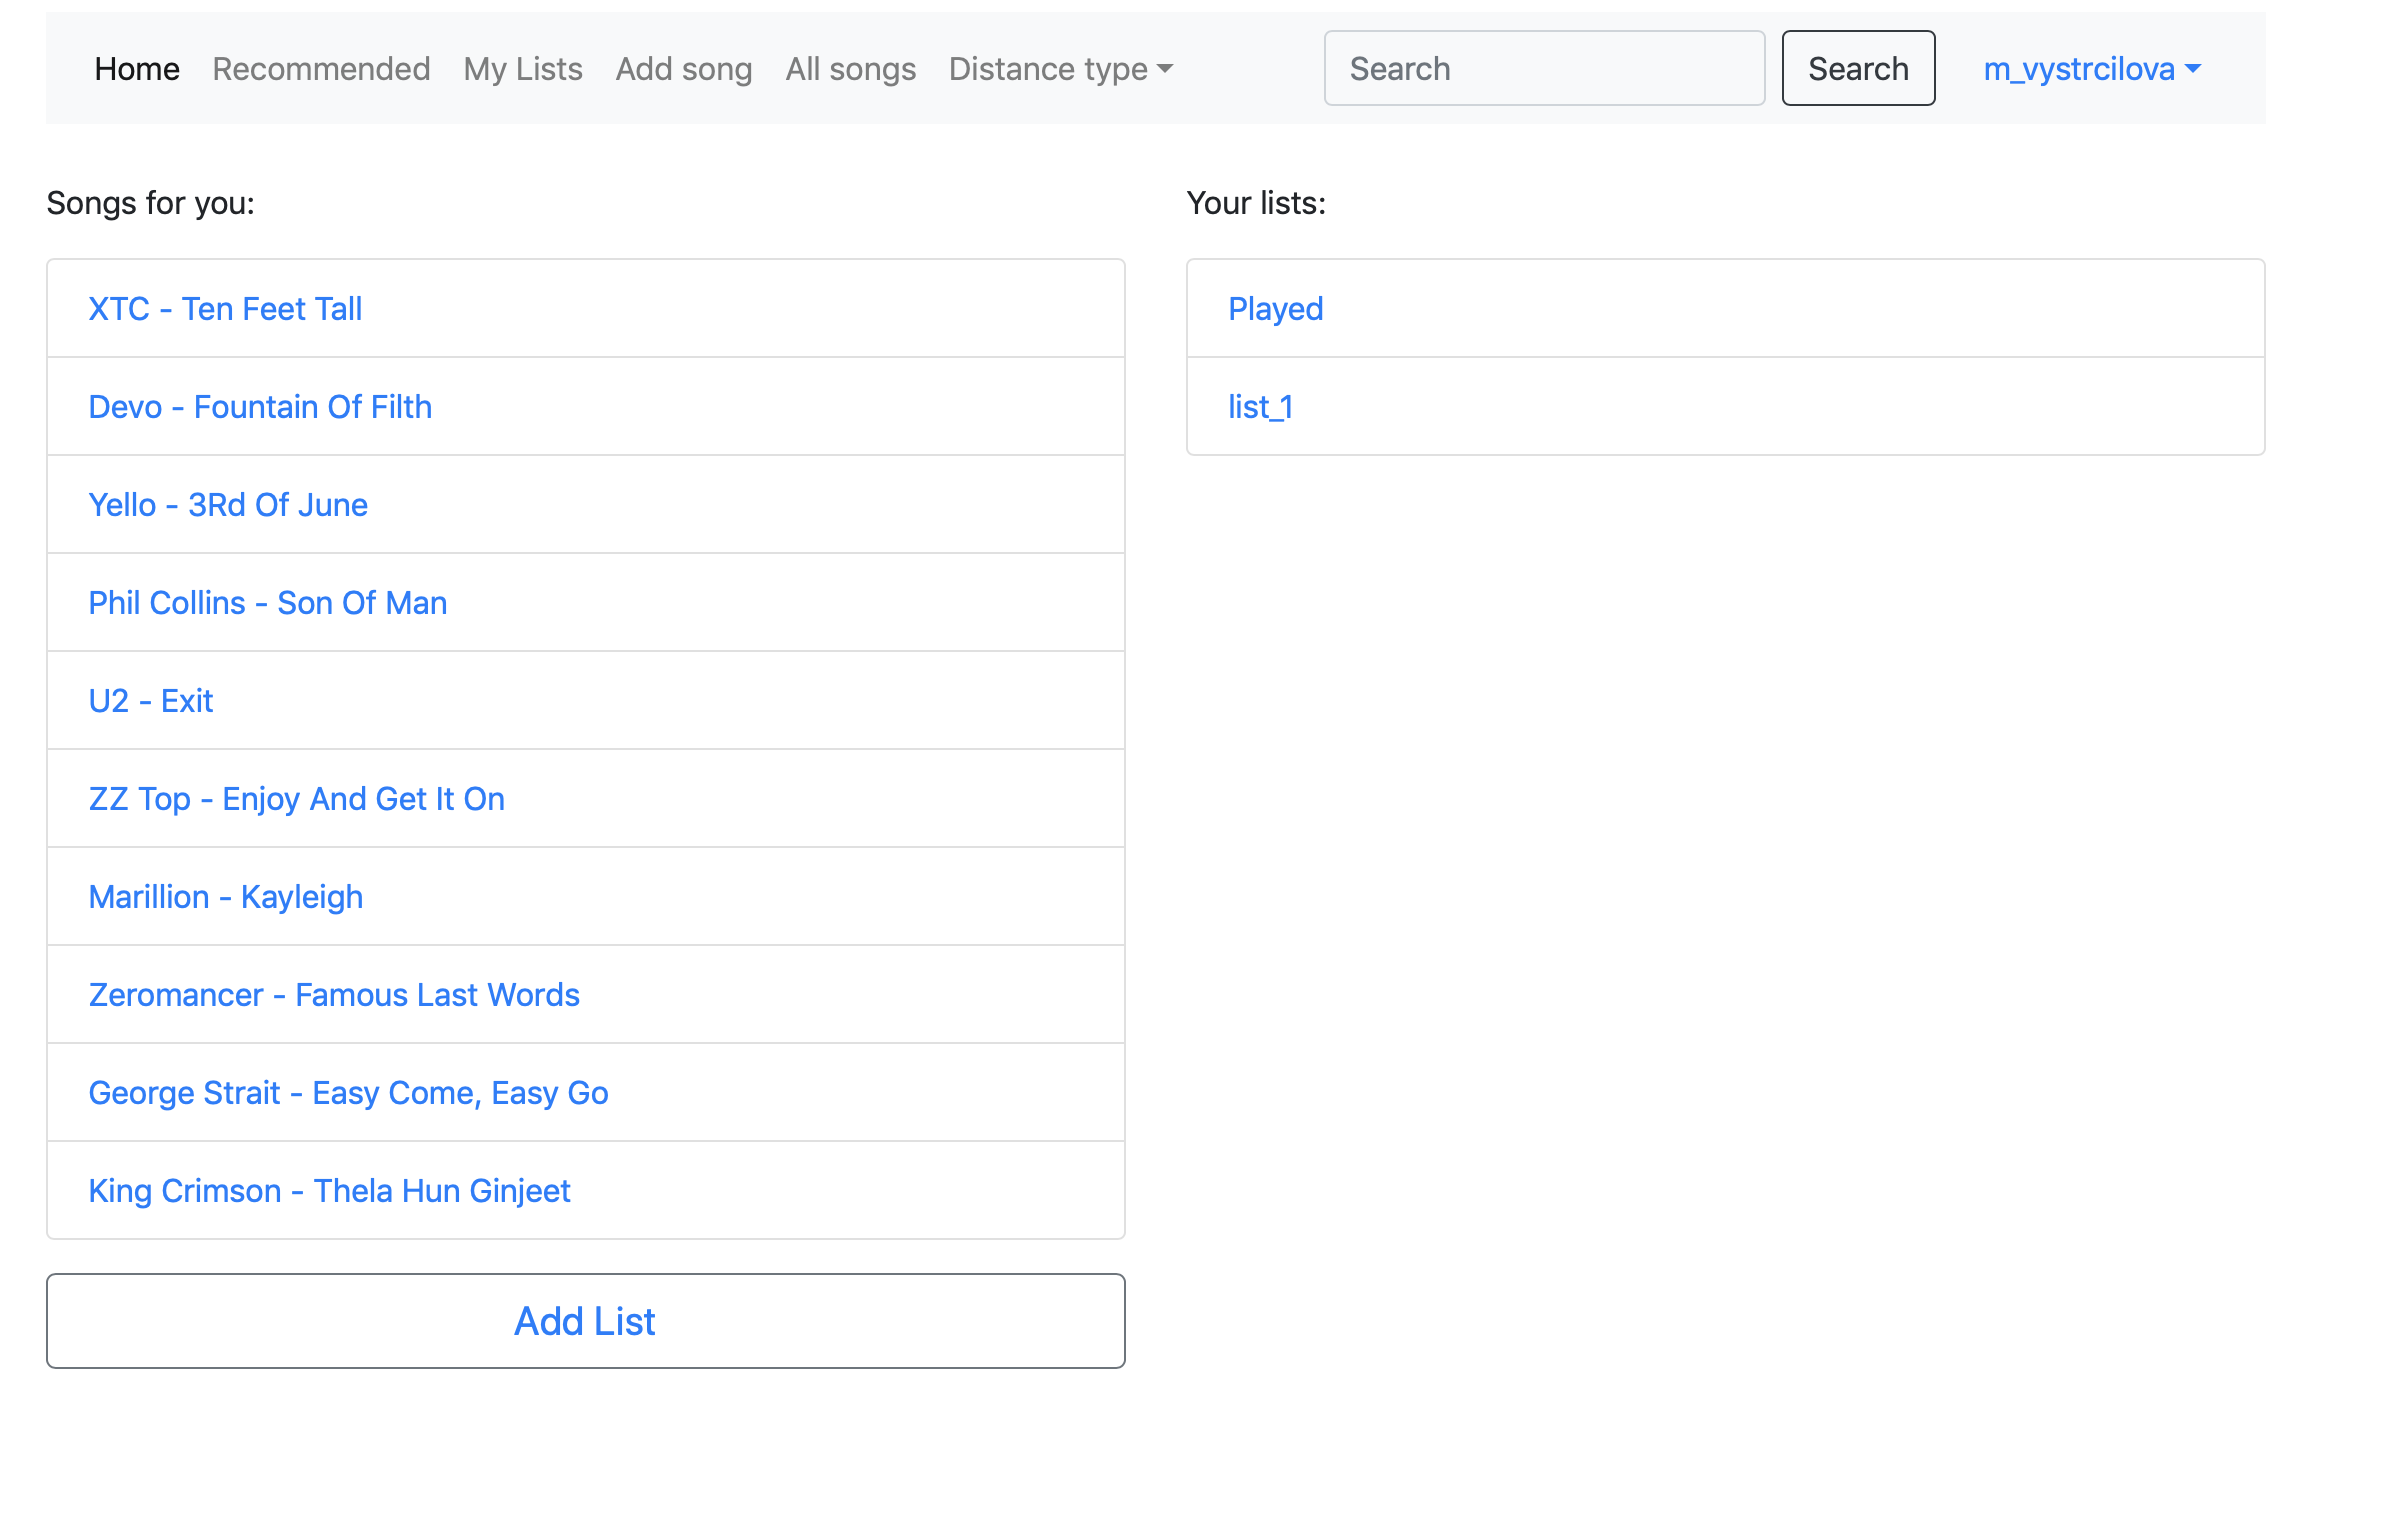
\includegraphics[width=1\linewidth]{./img/home_page.png}
	\caption{A screenshot of the homepage of the proposed web application}
	\label{fig:home_page}
\end{figure}

He can also go to his \textit{Recommended} page whose screenshot is in Figure \ref{fig:recommended_page} where he can see all the songs he played and top ten recommendations for him. Recommendations exclude disliked and played songs. Another thing illustrated in this Figure is the possibility to use the \textit{Distance type} drop-down menu and change the metrics based on which songs are recommended.
\begin{figure}[H]
    \centering
	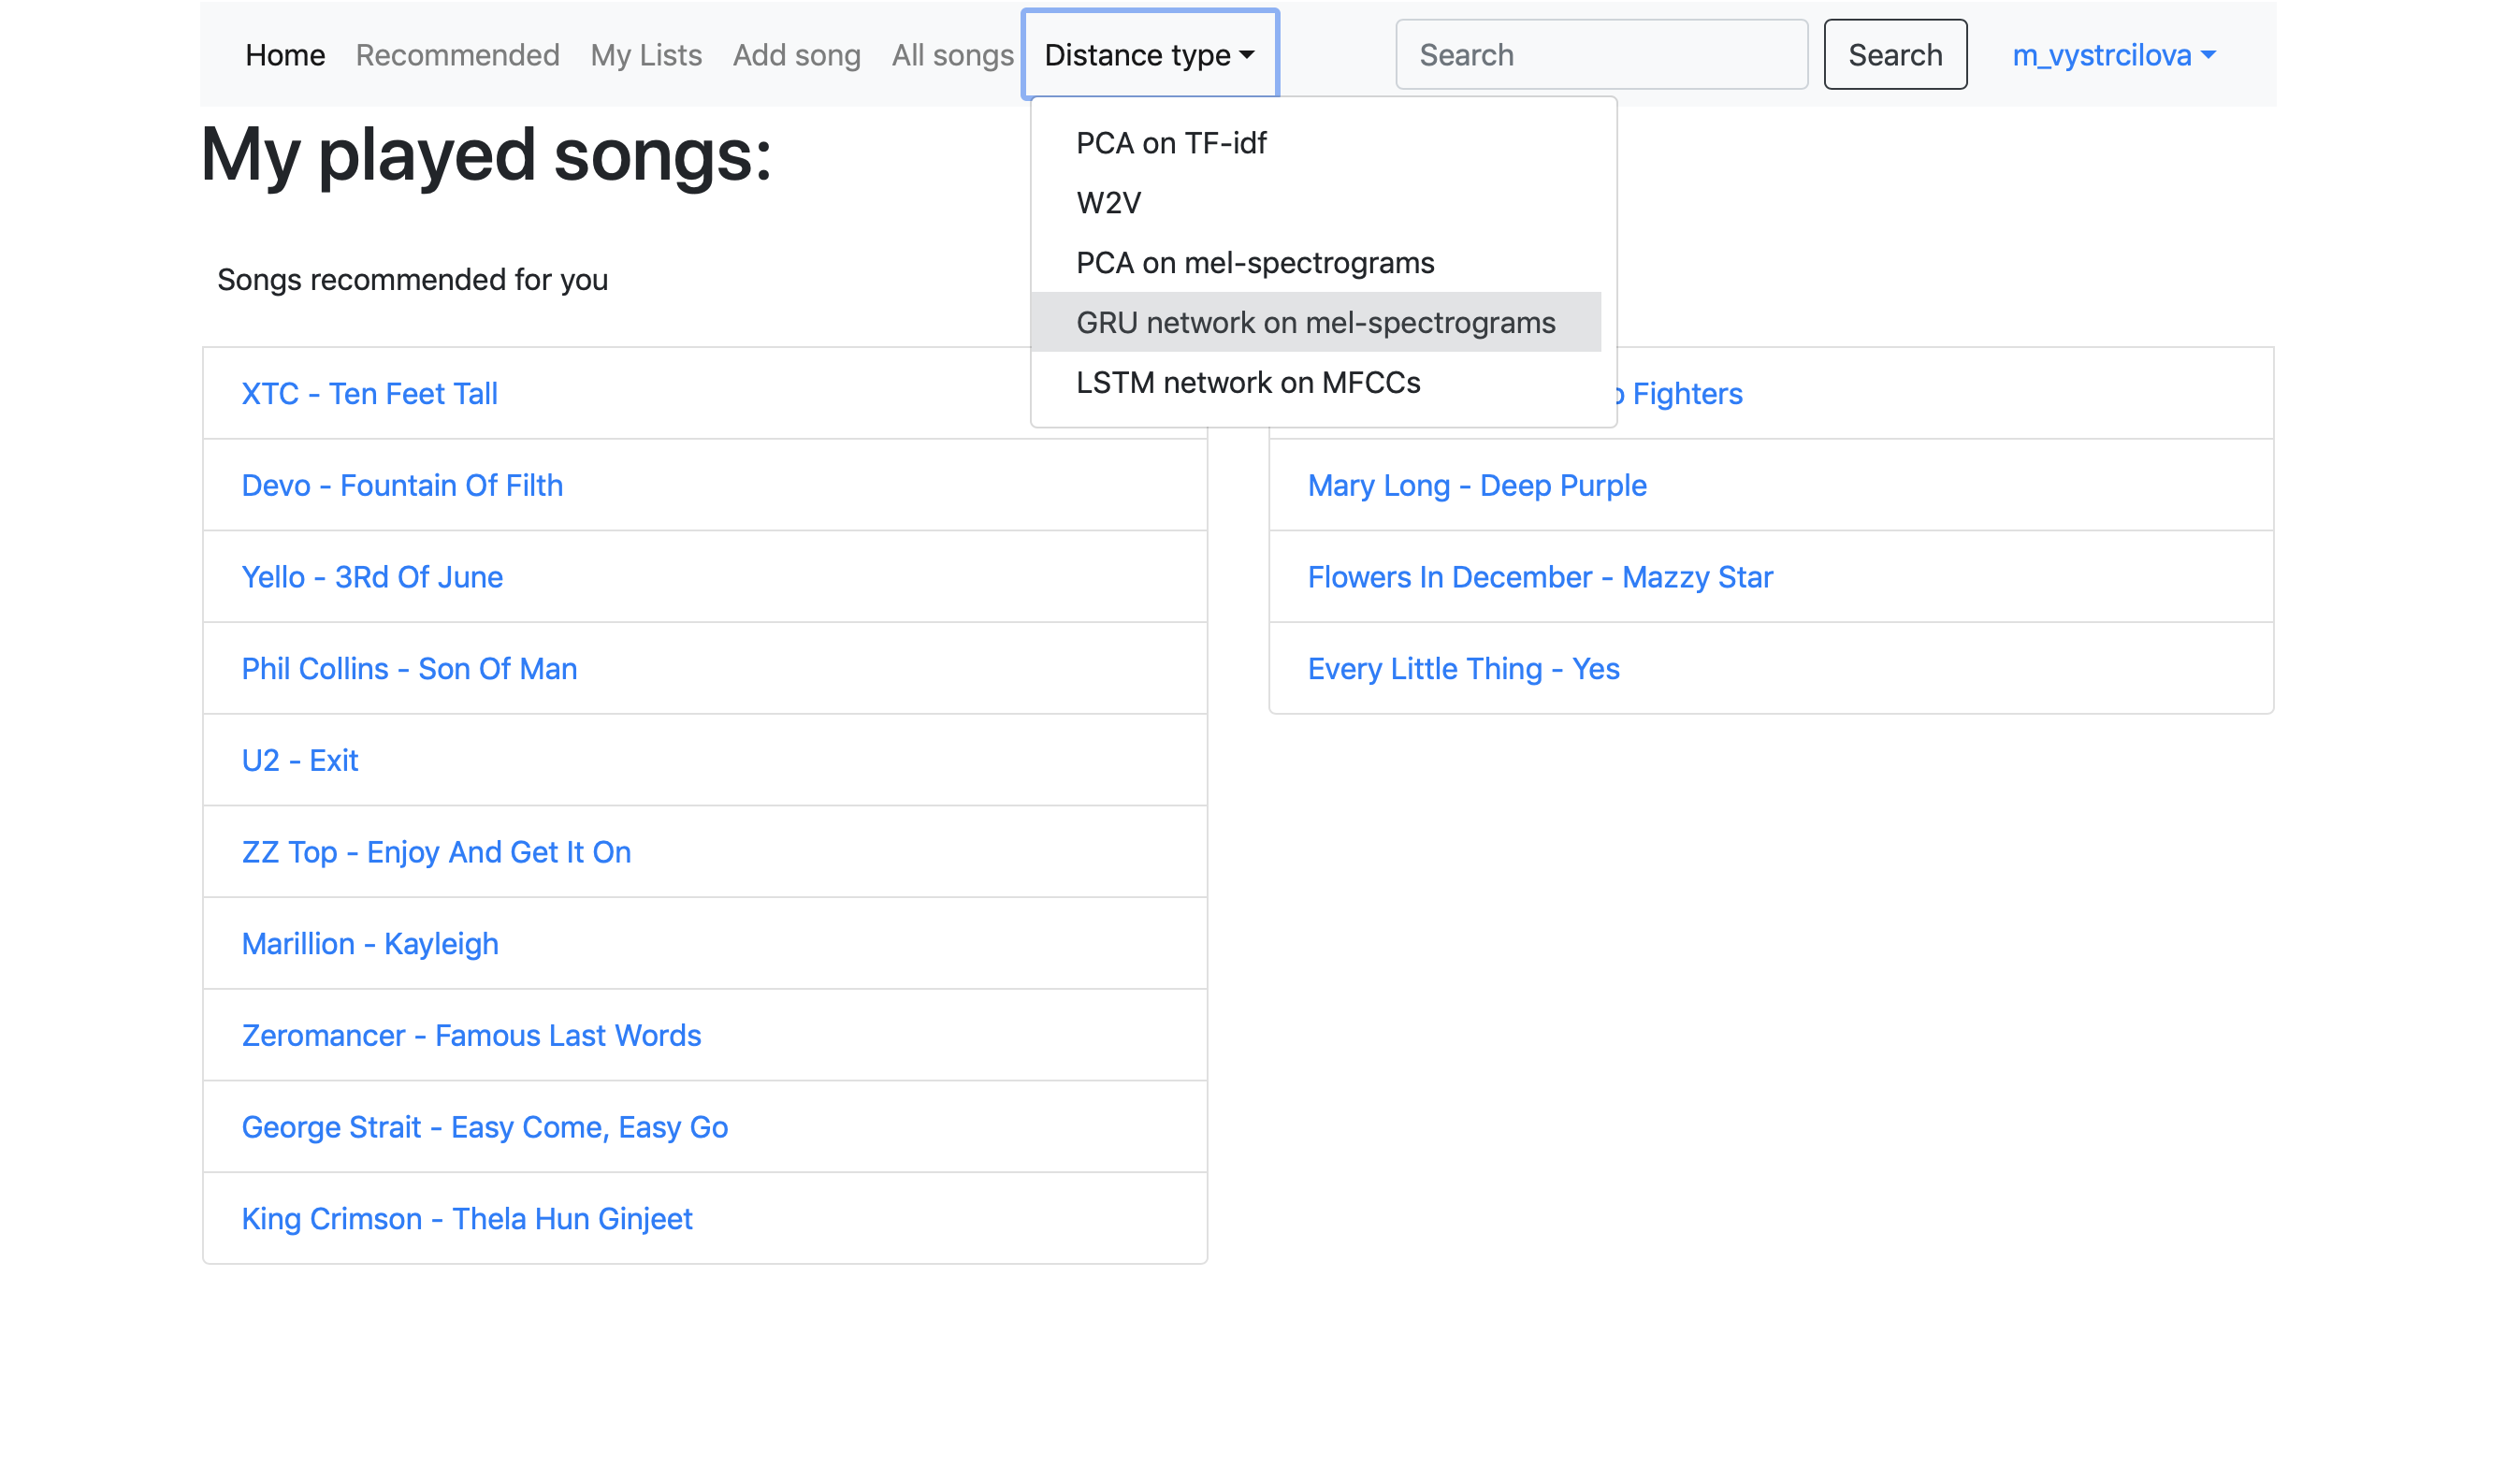
\includegraphics[width=1\linewidth]{./img/recommended_page.png}
	\caption{A screenshot of the Recommended page of the proposed web application with an active Distance type drop-down menu to change the distance based on which recommendations are calculated.}
	\label{fig:recommended_page}
\end{figure}
The \textit{My lists} page displays all lists he has created and top ten most similar songs for each of those lists including the complete list of songs he has played. The \textit{My lists} page displayed in figure \ref{fig:my_lists_page}.  \\
\begin{figure}[H]
    \centering
	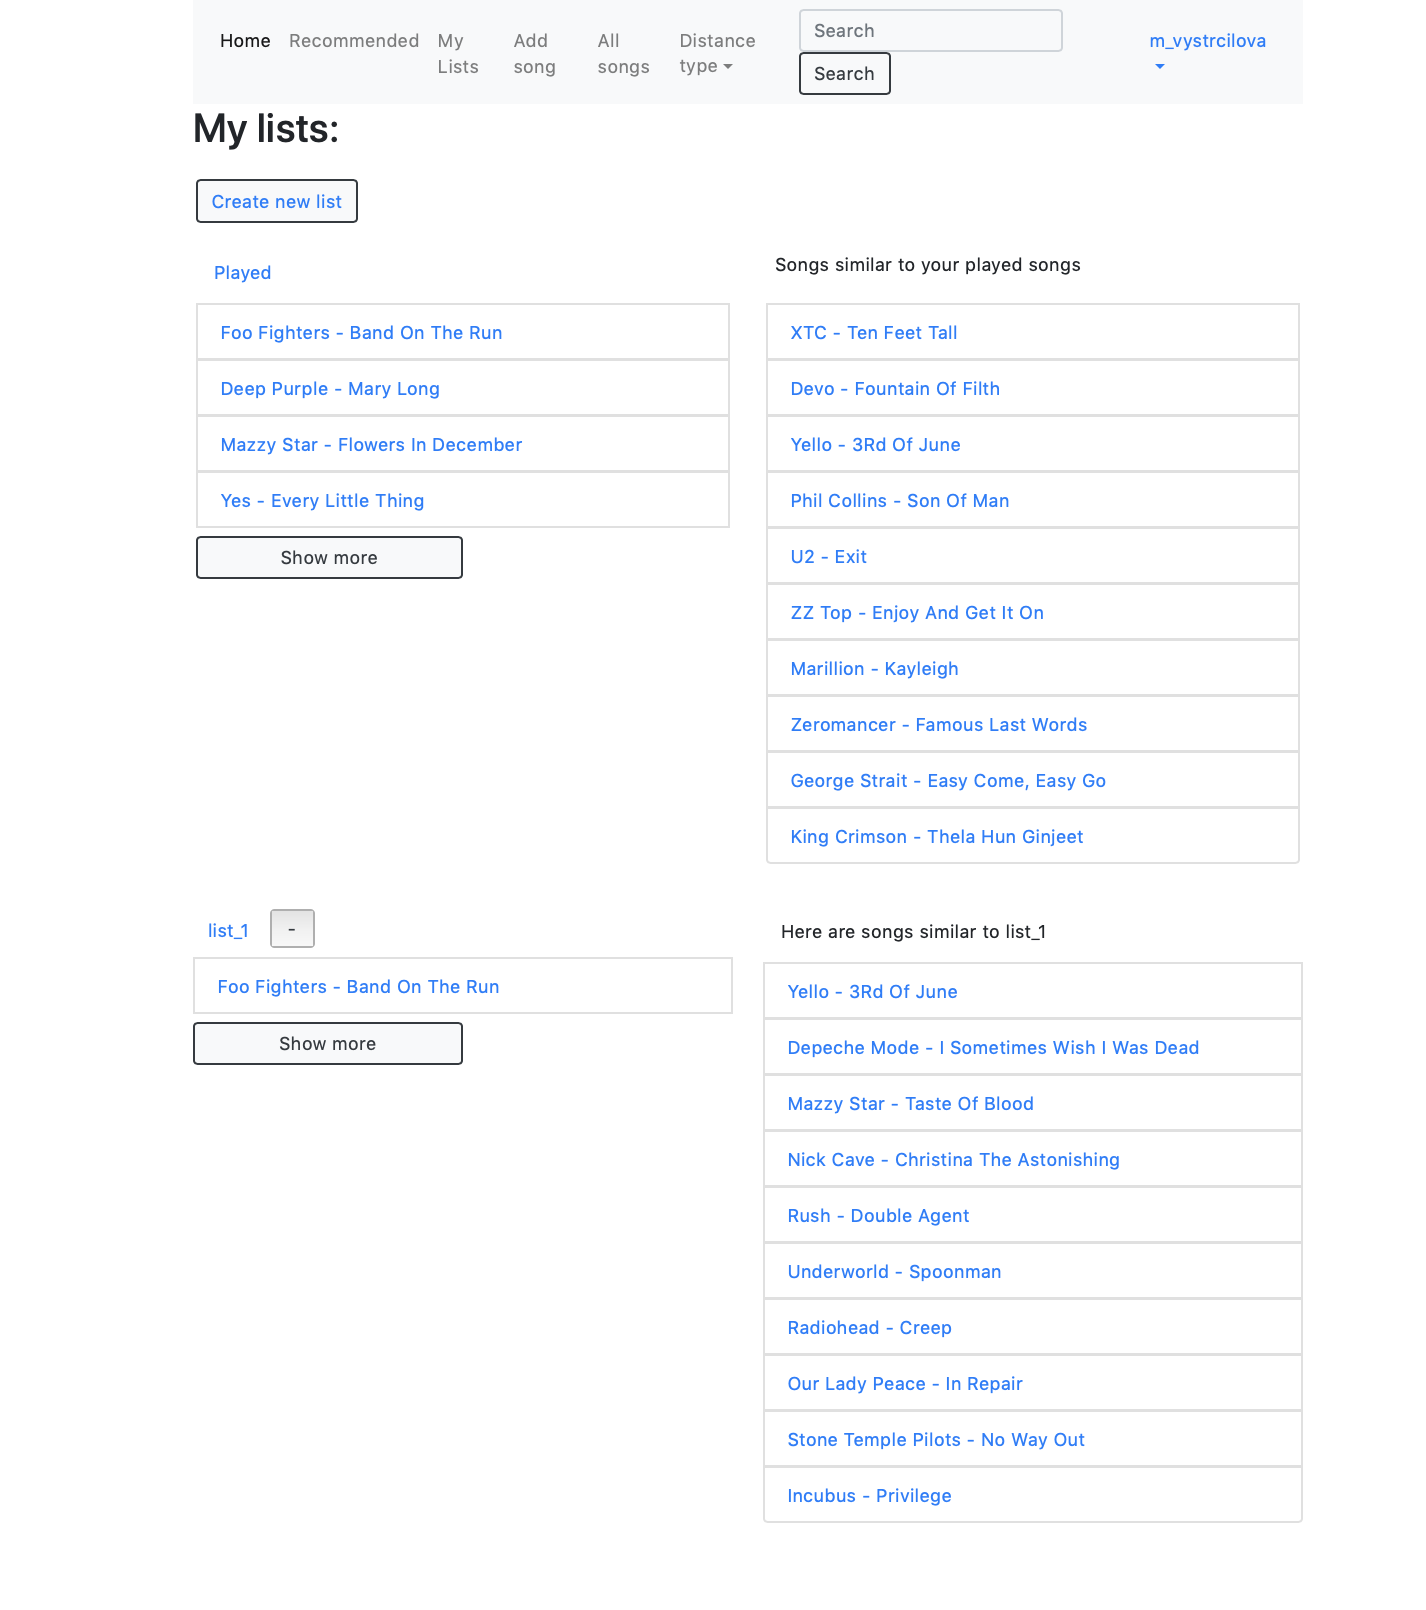
\includegraphics[width=1\linewidth]{./img/my_lists_page.png}
	\caption{A screenshot of the My lists page of the proposed web application.}
	\label{fig:my_lists_page}
\end{figure}
Next there is a possibility to add a song, which redirects the user to a form he fills out asking for a name of the song, the artist, the lyrics and a YouTube link as can be seen in Figure \ref{fig:add_song_form}. When he clicks add, this song is added to the database and has the same possibilities as the others.\\
\begin{figure}[H]
    \centering
	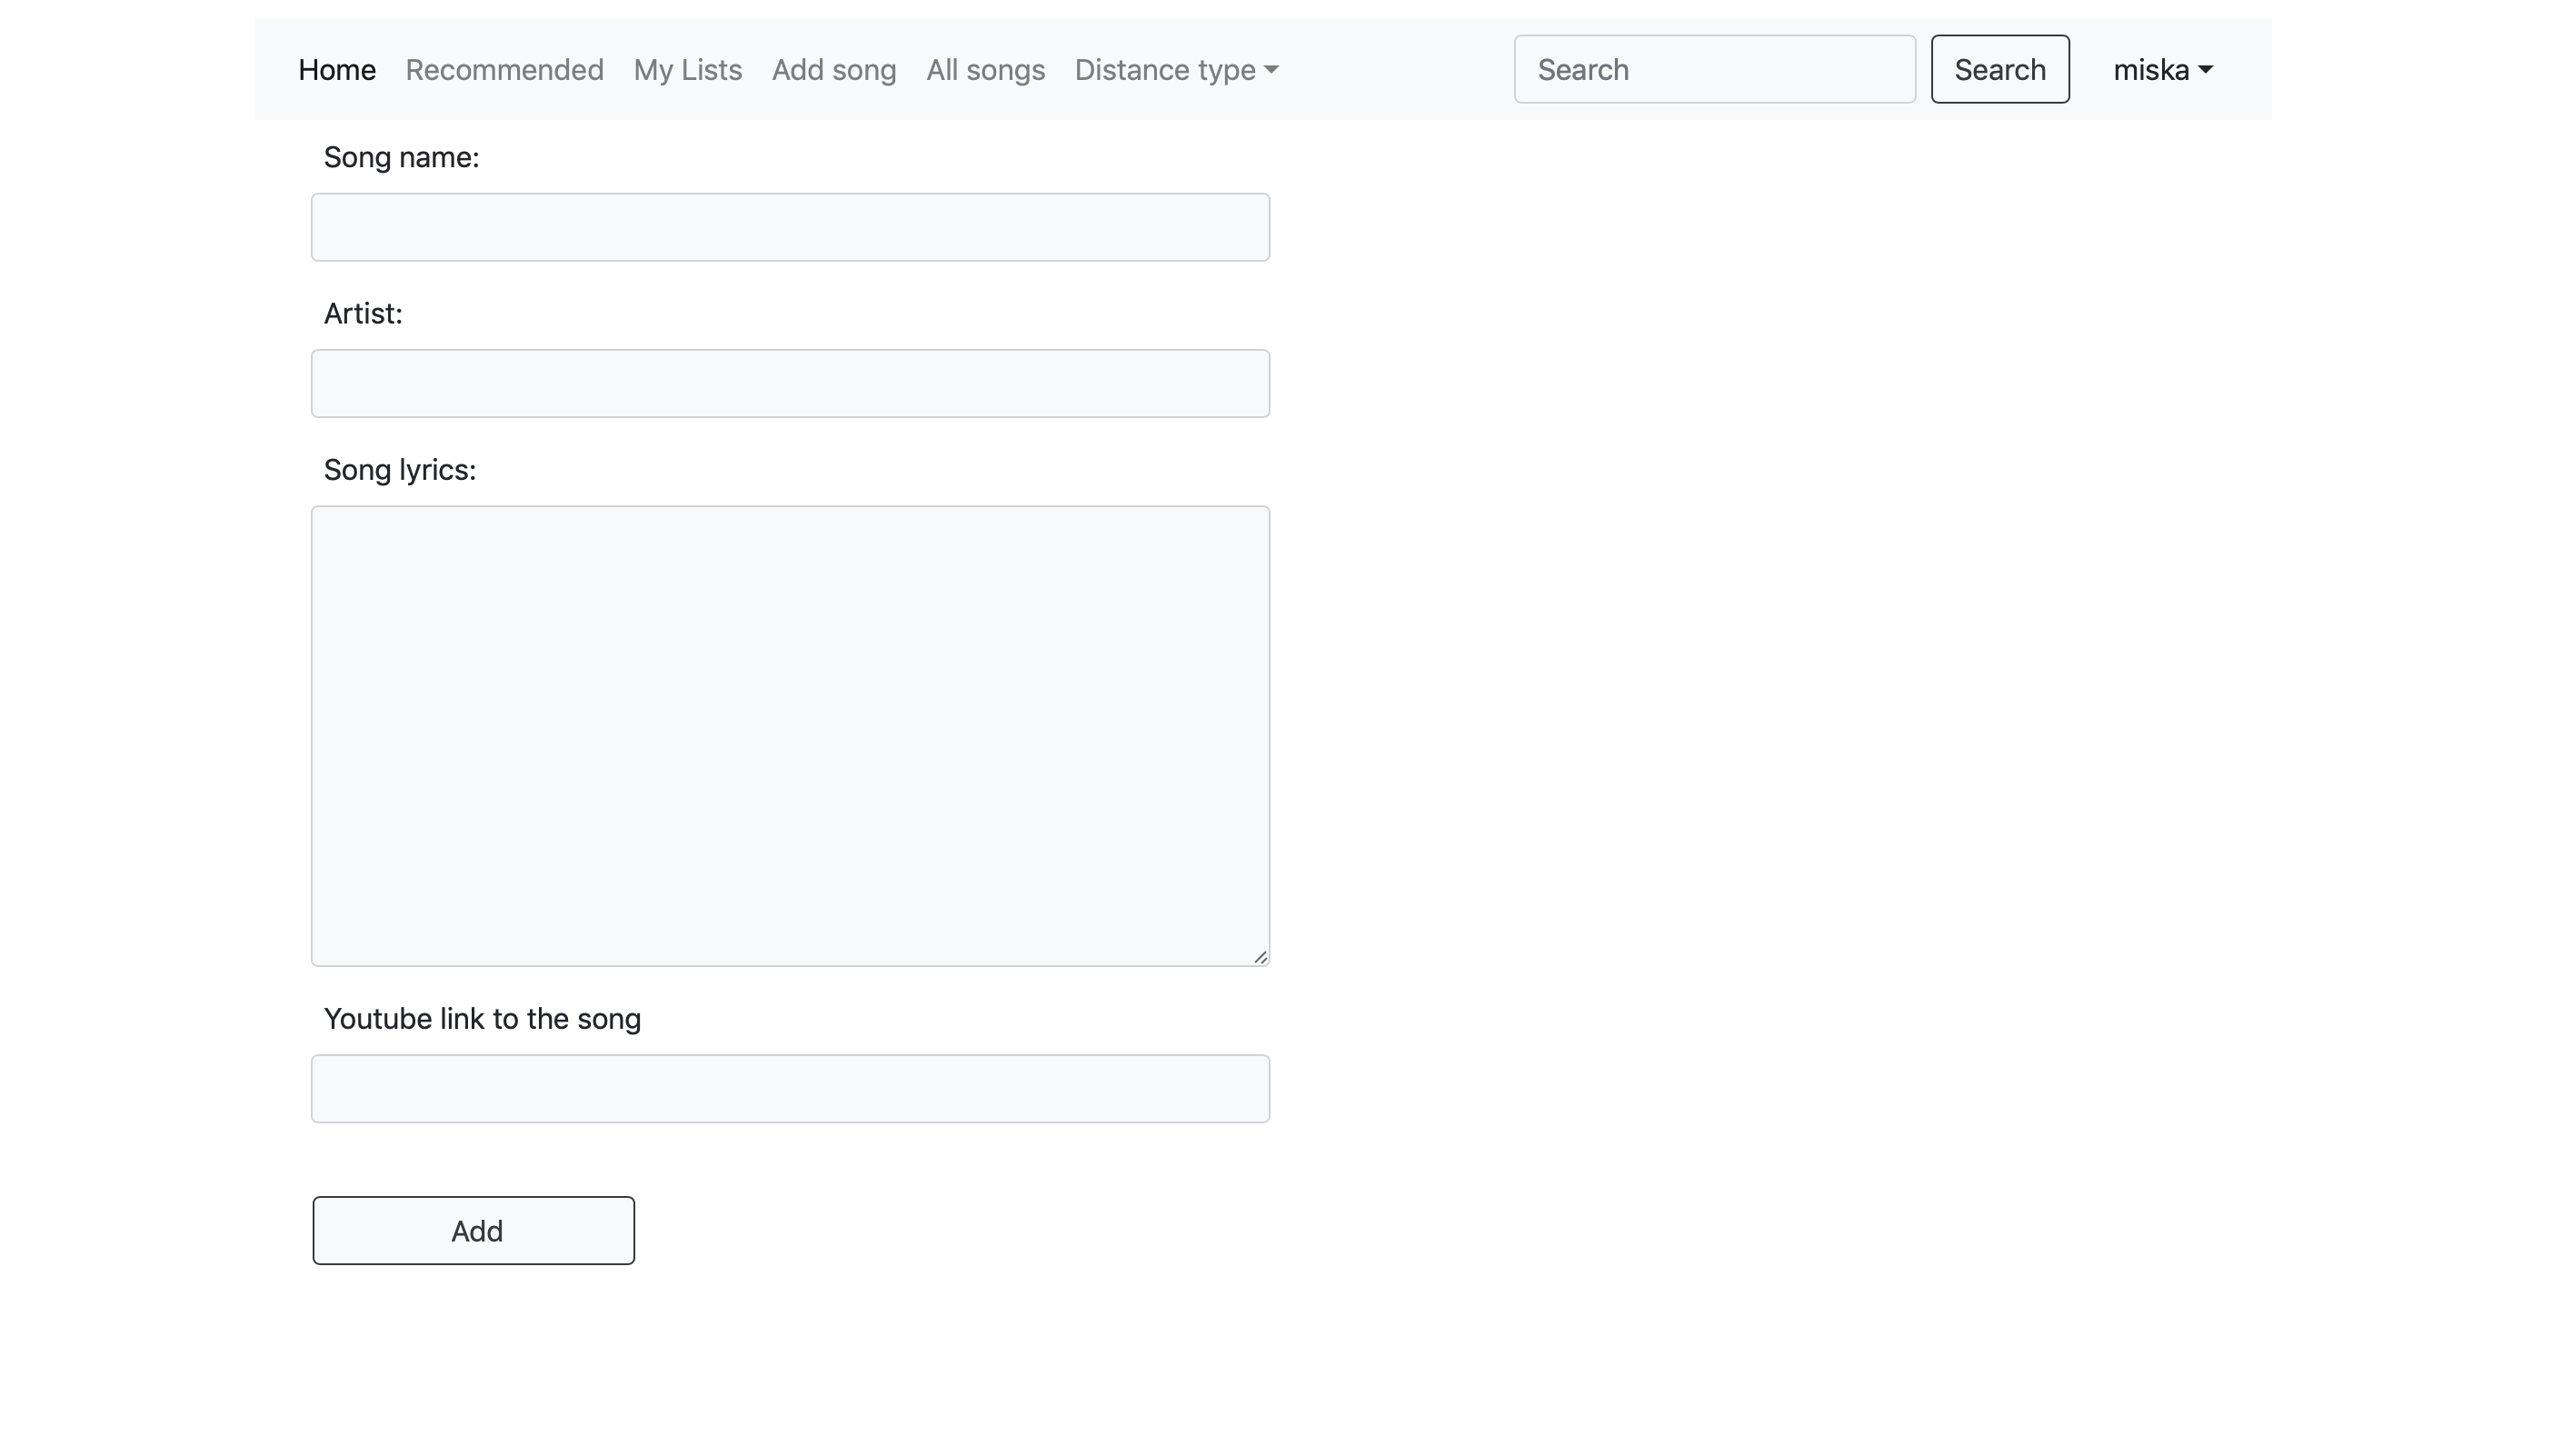
\includegraphics[width=1\linewidth]{./img/add_song_form.png}
	\caption{A screenshot of the All songs page of the proposed web application with an active drop-down menu.}
	\label{fig:add_song_form}
\end{figure}
The next button \textit{All songs} redirects to a page displaying songs that are in the database in a random order. The page can be seen in Figure \ref{fig:all_songs_view}. In the same Figure we can also see the drop-down menu where the user can logout, delete his account or go to a web page \textit{About this application} where the different distance metrics are described.
\begin{figure}[H]
    \centering
	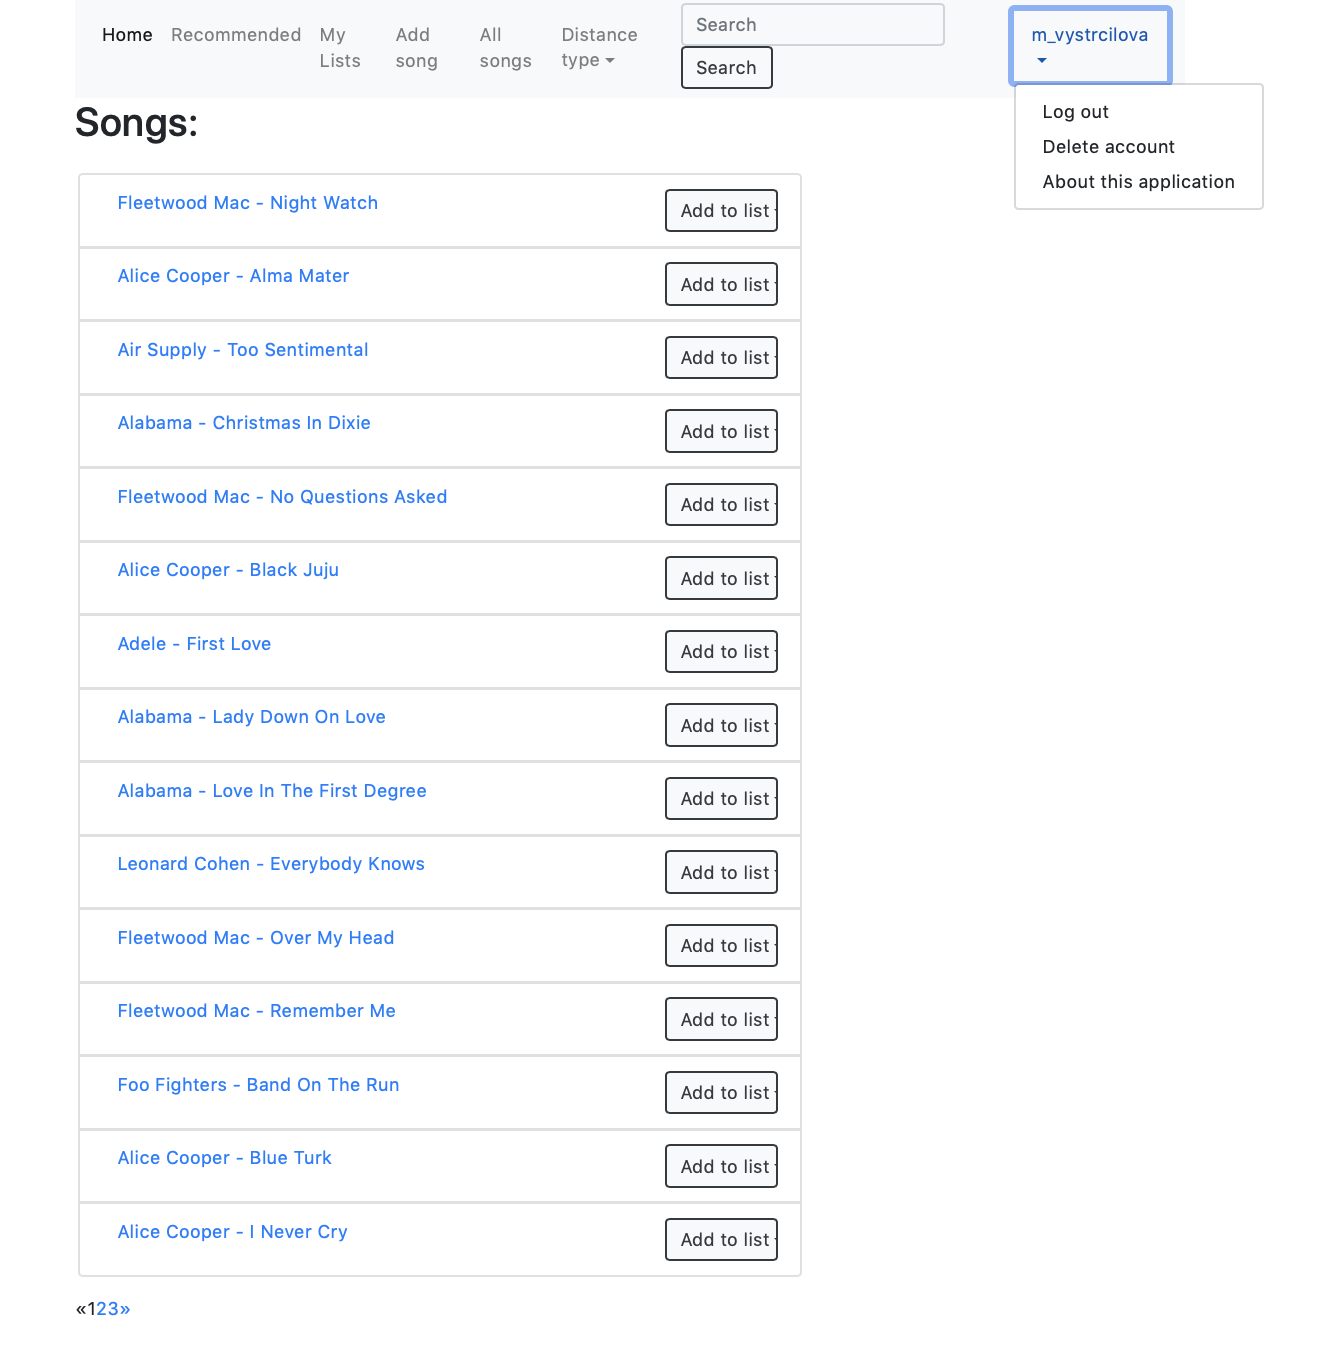
\includegraphics[width=1\linewidth]{./img/all_songs_page.png}
	\caption{A screenshot of the All songs page of the proposed web application with an active drop-down menu.}
	\label{fig:all_songs_page}
\end{figure}
There is also a search bar, where one can search for songs based on title and artist. Illustrative results for the search of "Nirvana" can be seen in \ref{fig:search_results} \\
\begin{figure}[H]
    \centering
	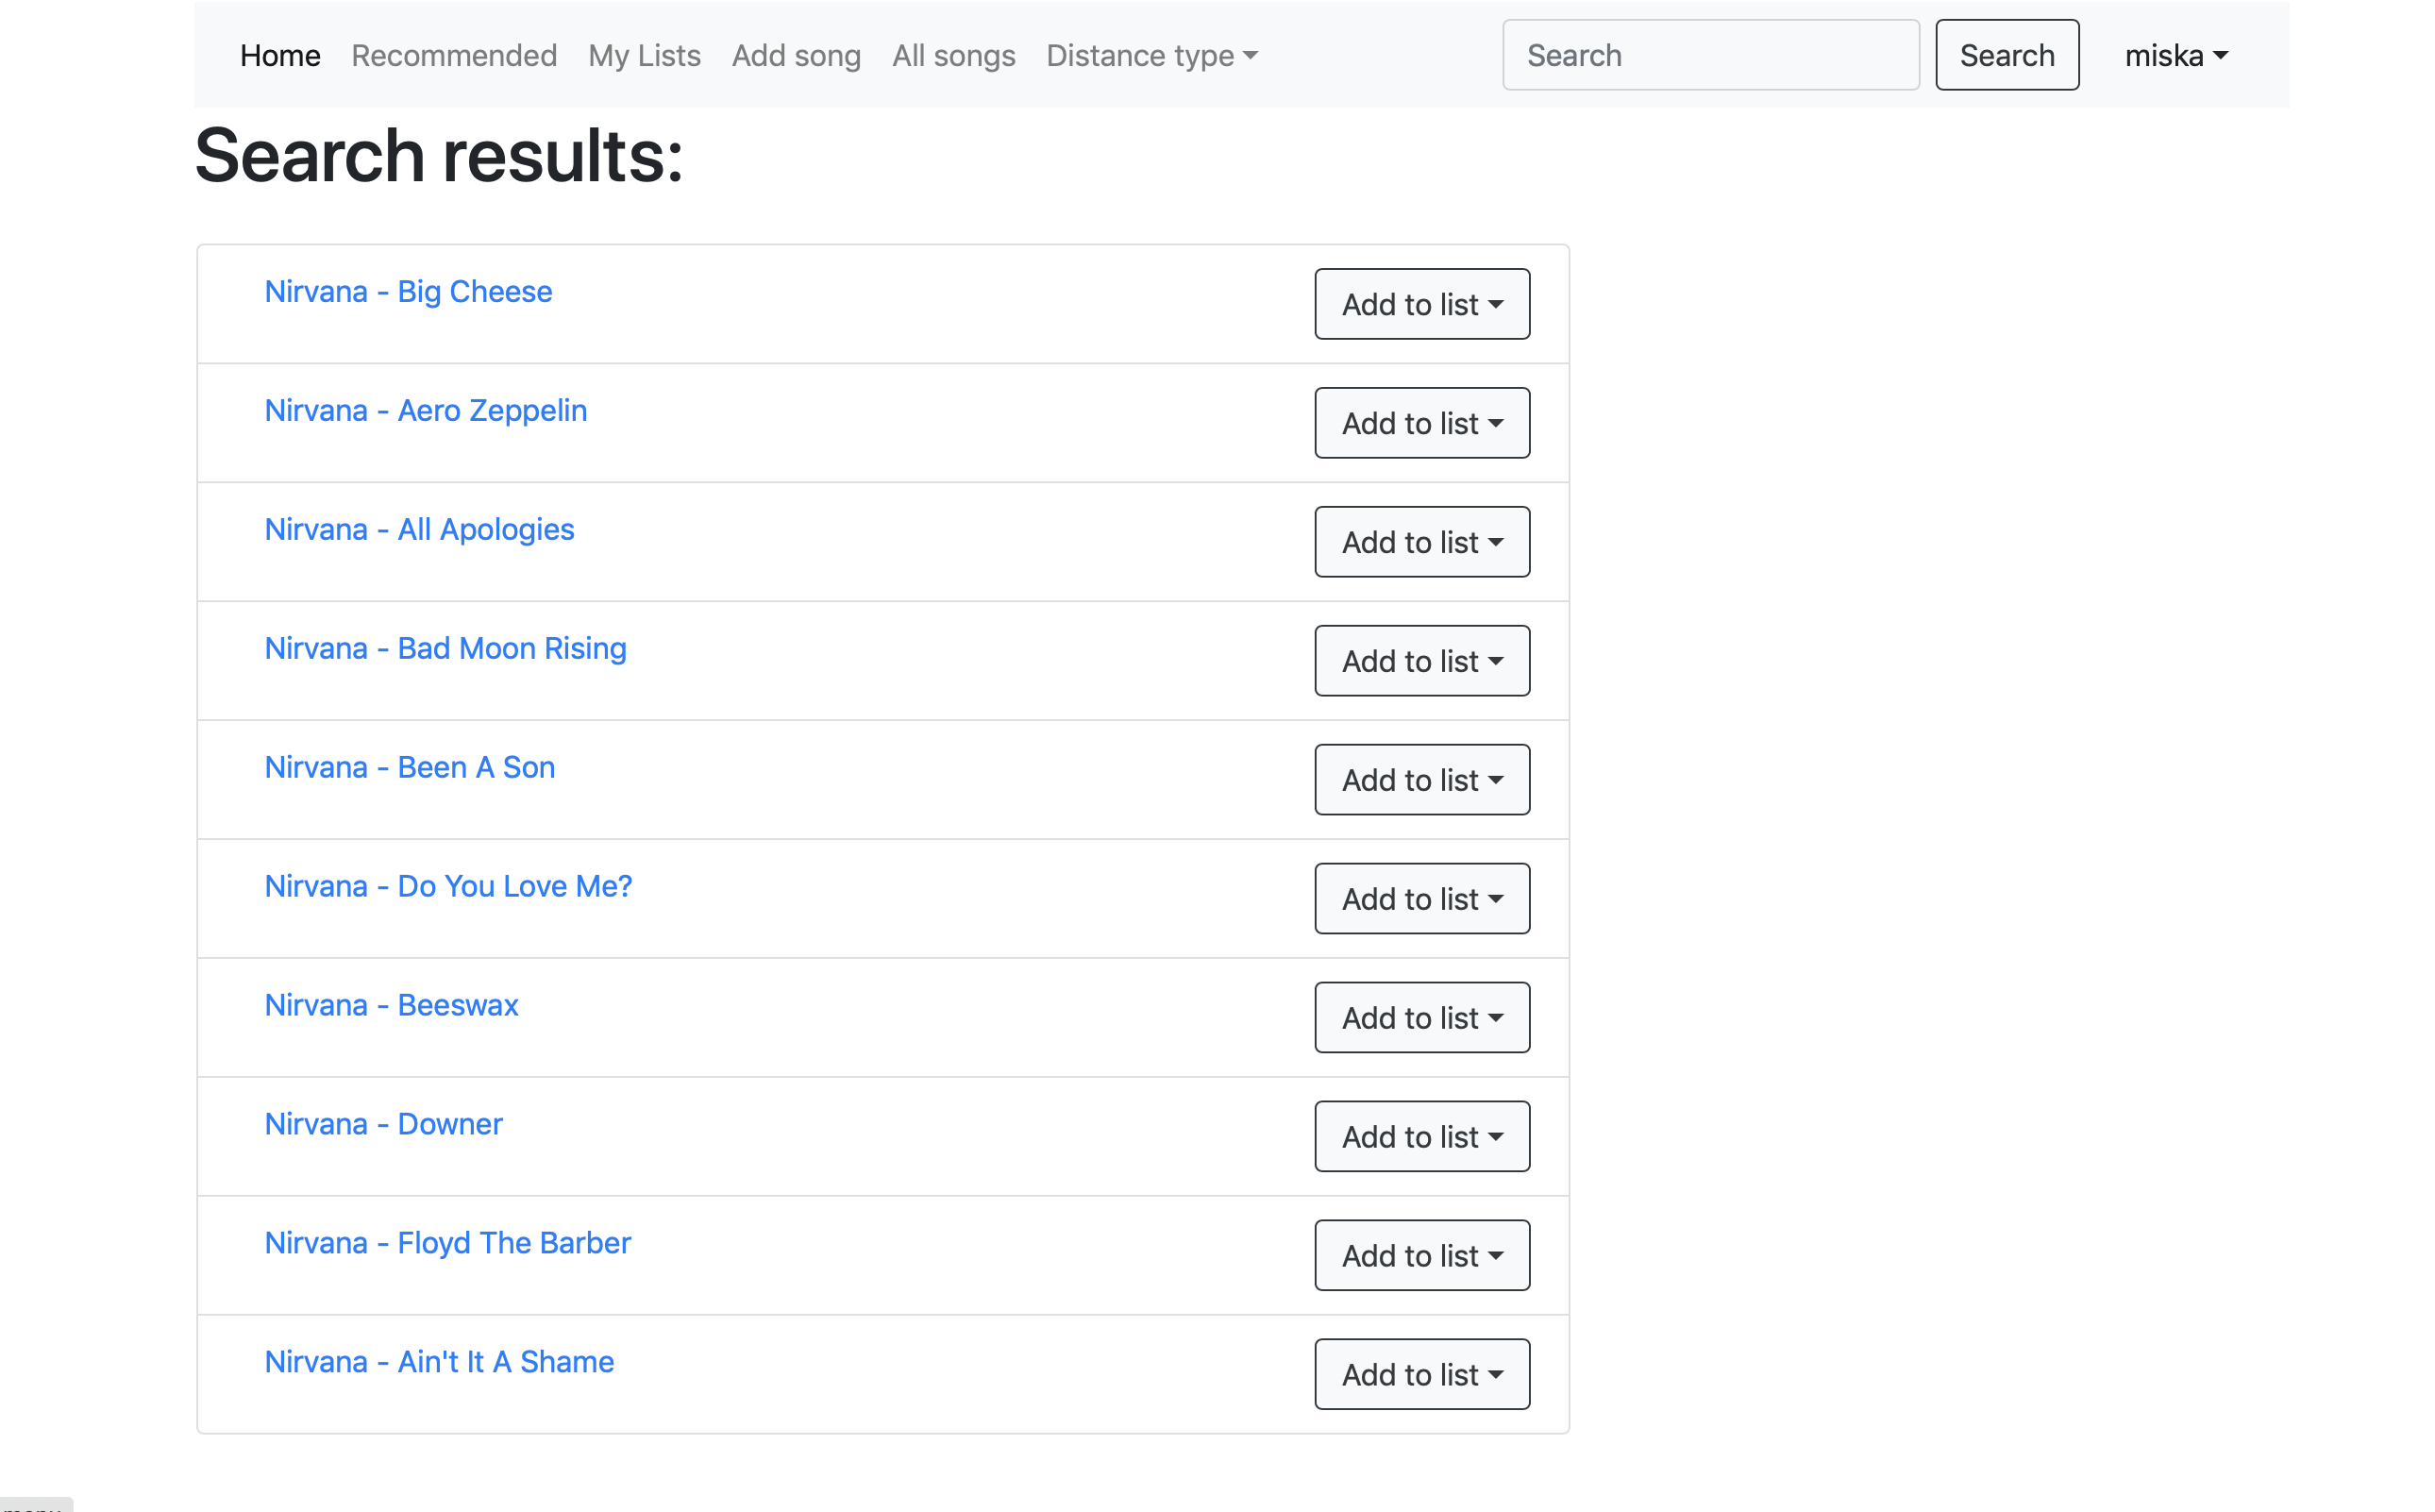
\includegraphics[width=1\linewidth]{./img/search_results_page.png}
	\caption{A screenshot of the All songs page of the proposed web application with an active drop-down menu.}
	\label{fig:search_results_page}
\end{figure}
A detail page of a songs allows the user play the audio of the song. He can also like or dislike the songs. If a song is disliked, it does not appear in recommendations and is not included into similarity calculations. There is also the possibility to add a song to a list.
Right to the song, there are its ten most similar songs. Here even disliked and played songs are included. A illustrative \textit{SongDetail page} of the song "" is displayed in Figure \ref{fig:song_detail_page}. \\
\begin{figure}[H]
    \centering
	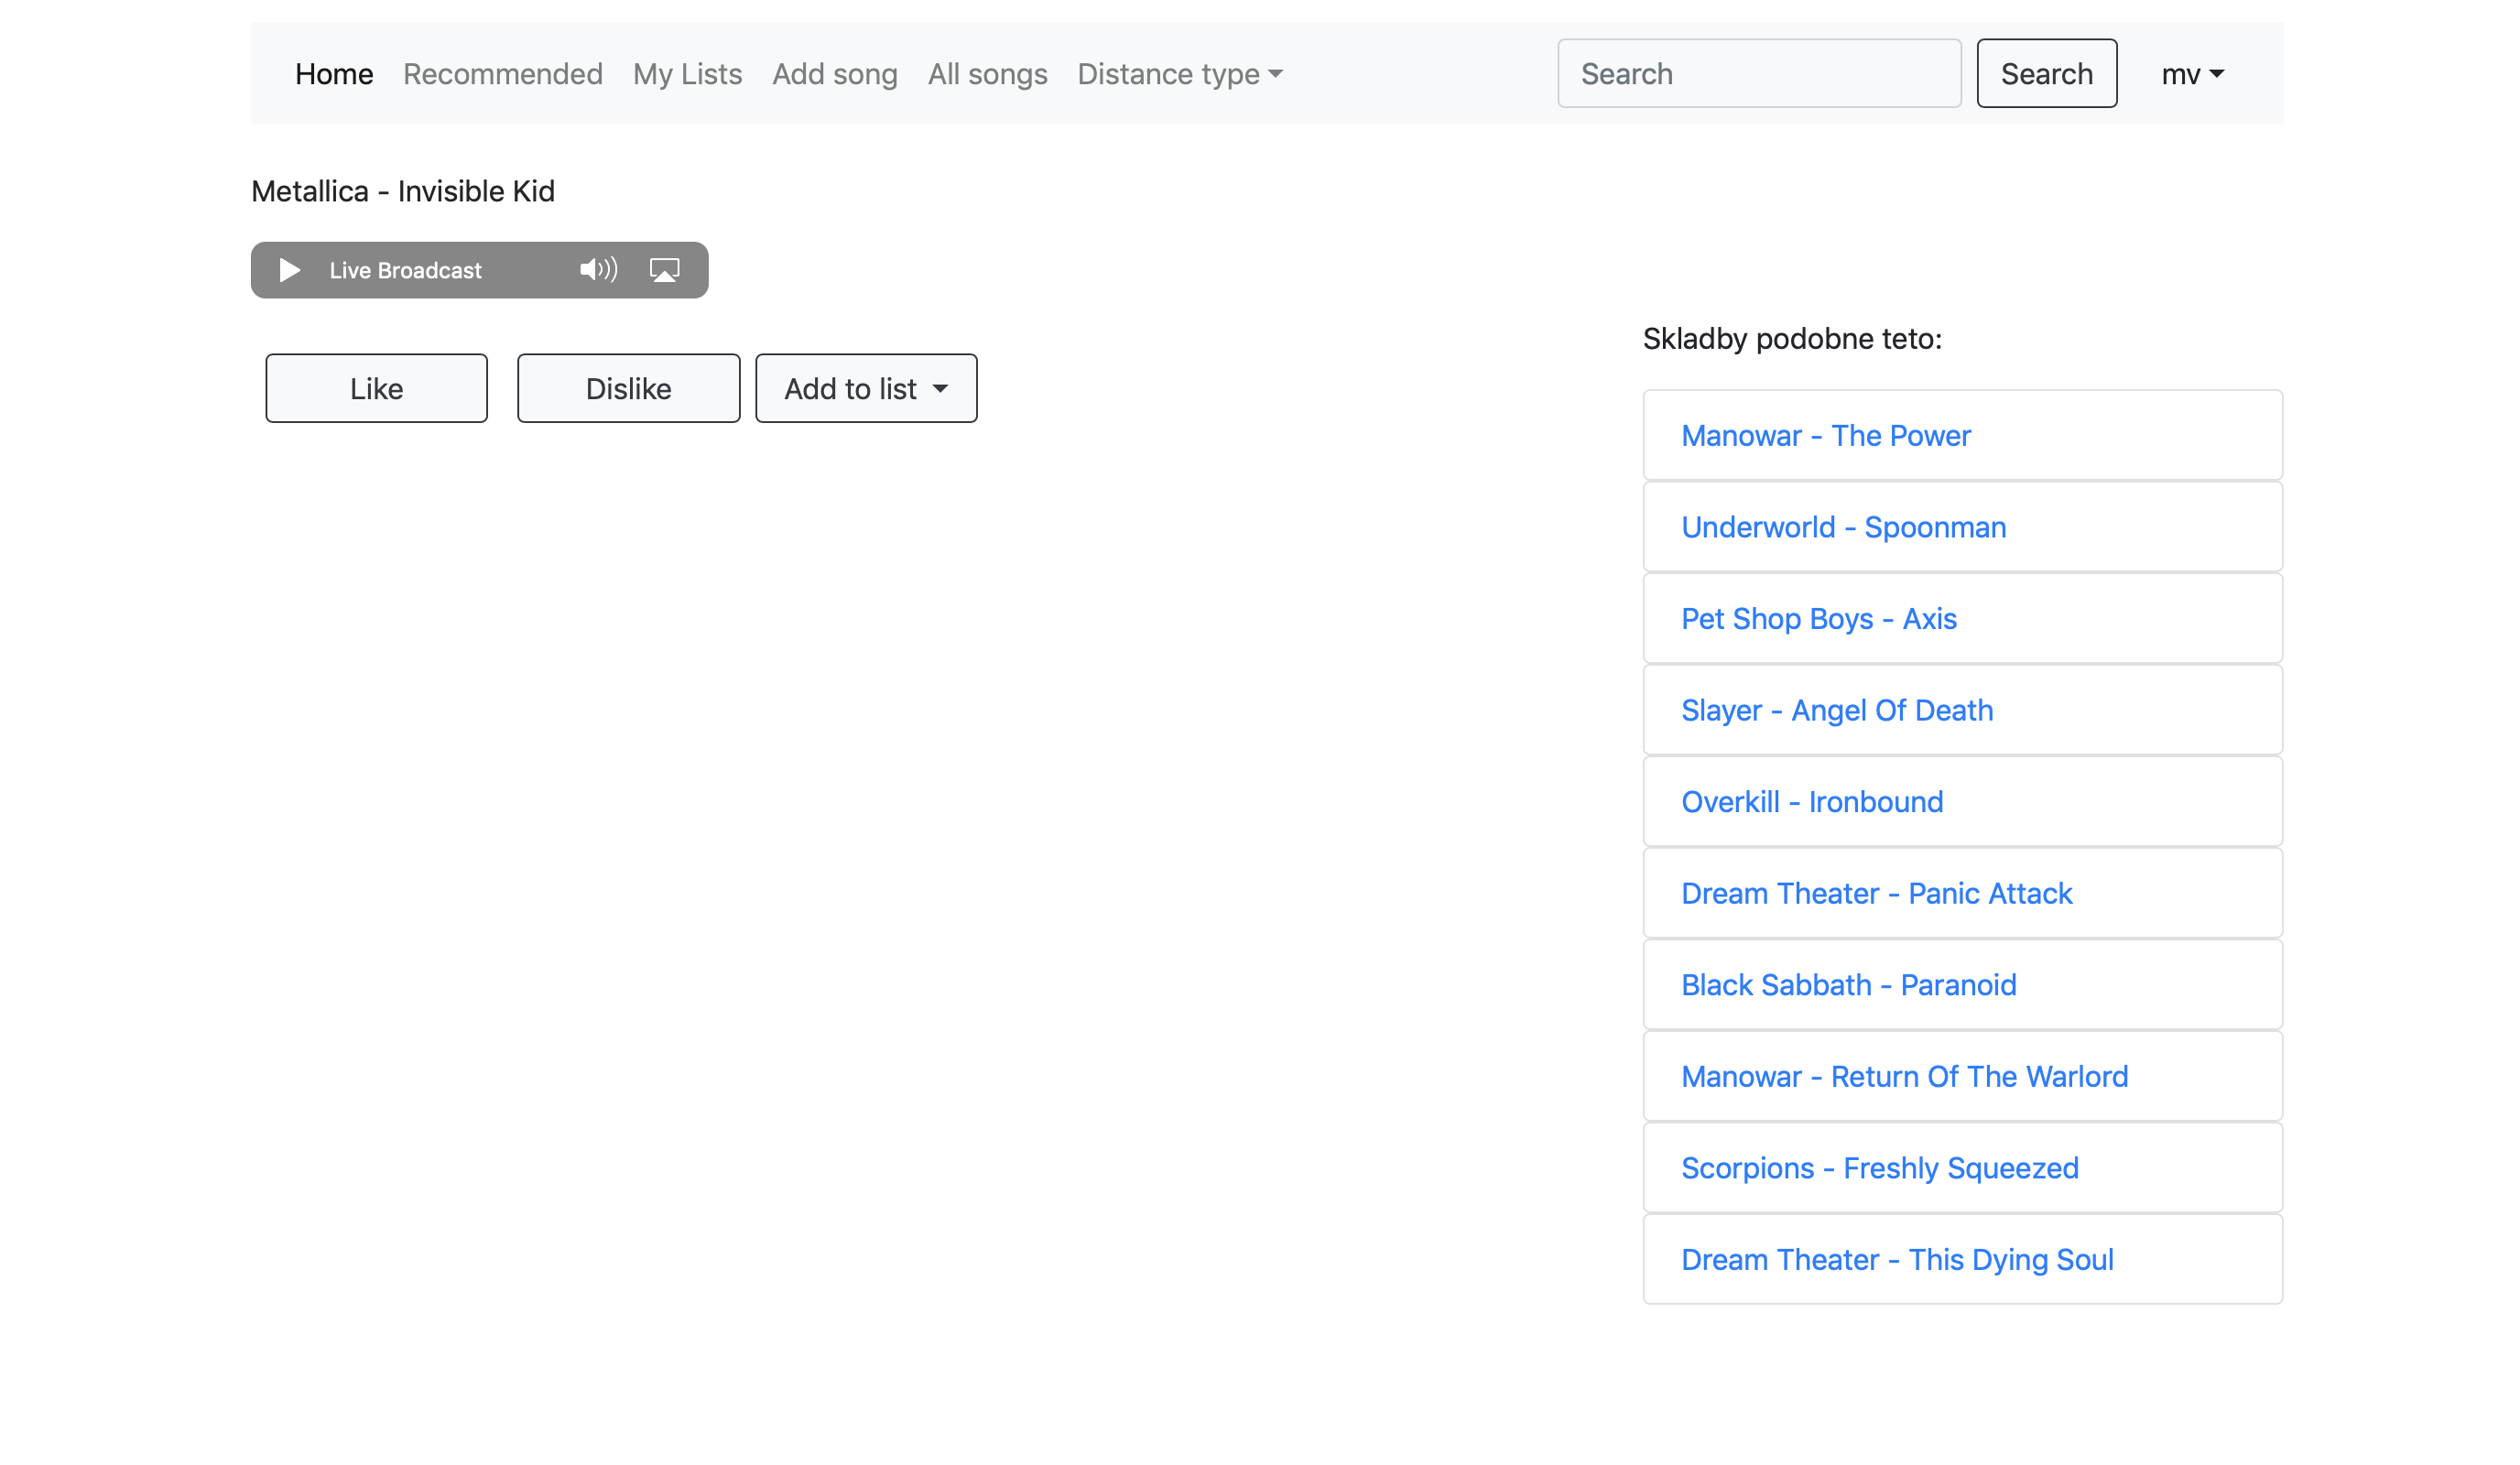
\includegraphics[width=1\linewidth]{./img/song_detail_page.png}
	\caption{A screenshot of the All songs page of the proposed web application with an active drop-down menu.}
	\label{fig:song_detail_page}
\end{figure}
A detail page of a list allows the user to see top ten most similar songs to this list and all the songs he has added to the particular list. The top ten similar songs again exclude played songs and disliked songs. \\




